\graphicspath{{./figs/repo/}{./figs/}}
\section{Policy based Reinforcement Learning}

\begin{frame}{Value Function Approximation}
    %{{{
    \begin{center}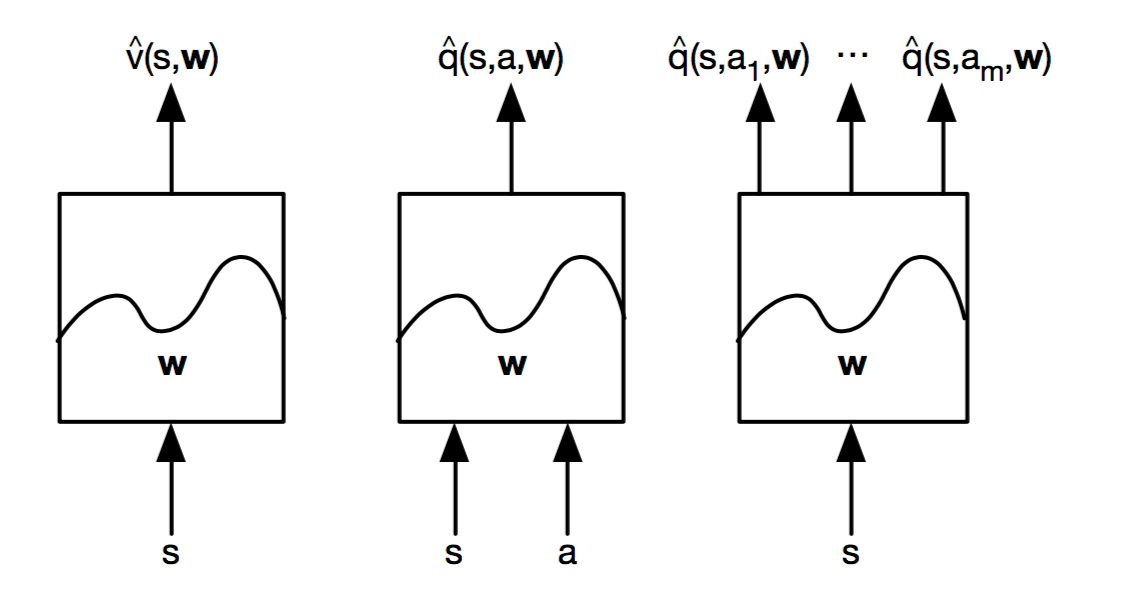
\includegraphics[width=.6\textwidth]{fun_app}\end{center}
    \begin{itemize}
        \item Tablular methods: impossible to record all states for real word problems 
        \item Function approximation: generalize from seen states to unseen states
    \end{itemize}
\end{frame}

\begin{frame}{Value Function Approximation}
    \begin{itemize}
        \item Goal: find parameter vector $w$ minimising mean-squared error between approximate value function $\hat{v}(S,w)$ and true value function $v_{\pi}(S)$
        \begin{align}
            \label{eq:1}
            J(w) = ||v_{\pi}(S)-\hat{v}(S,w)||_2^2
        \end{align}
        \item Stochastic gradient descent
        \begin{align}
            \label{eq:1}
            \Delta w = \alpha (v_{\pi}(s)-\hat{v}(S,w)) \nabla_{w}\hat{v}(S,w)
        \end{align}
        \item In reality we don't have the true value function $v_{\pi}(S)$\\
        \vspace{0.2cm}
        \hspace{0.5cm}$\bullet$ For Monte-Carlo, use discounted return $G_t$\\
        \vspace{0.2cm}
        \hspace{0.5cm}$\bullet$ For TD, use $R_{t+1}+\lambda \hat{v}(S_{t+1},w)$
        
    \end{itemize}
\end{frame}

\begin{frame}{Deep Q-Networks (DQN)}
    %{{{
    \begin{itemize}
        \item Take action $a_t$ according to $\epsilon$-greedy policy
        \item Store transition $(s_t,a_t,r_{t+1},s_{t+1})$ in memory $D$
        \item Sample random mini-batch of transitions $(s,a,r,s')$ from $D$
        \item Compute Q-learning targets w.r.t. old, fixed parameters $w^-$
        \item Optimise MSE between Q-network and Q-learning targets
            \begin{align}
                \label{eq:2}
                L(w) = \mathrm{E}_{s,a,s,r' \sim D_i}[(r+\gamma \max_{a'} Q(s',a';w^-)-Q(s,a;w))^2]
            \end{align}
        \item Two important tricks in ensuring convergence: experience replay and fixed target

    \end{itemize}
\end{frame}


\begin{frame}{Deep Q-Networks(DQN): play games in OpenAI gym}
    %{{{
    \begin{center}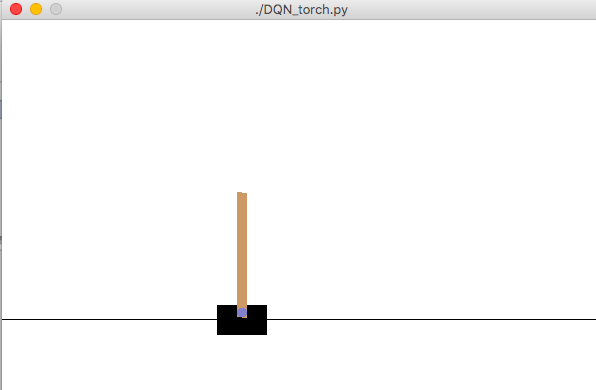
\includegraphics[width=.4\textwidth]{pole}\end{center}
    \begin{itemize}
        \item States are represented by 4-element tuples (position,cart velocity,angle,tip velocity)
        \item Actions can be either moving left or right
        \item Function approximator is a feed foward neural network 
        \item 1 hidden layer with 10 neurons, 2 output neurons representing value estimation for two actions
        \item Implemented using torch and tensorflow, can stay alive for 1 minute
    \end{itemize}

\end{frame}

\begin{frame}{Policy based method}
    Value based method (previous sildes):
    \begin{itemize}
        \item Main focus is on state-action value evaluation
        \item Policy improvement is based on greedy or $\epsilon$-greedy strategy w.r.t state-action values
        \item Return deterministic policy
    \end{itemize}\vspace{0.5cm}
    Policy based method (slides after this page):
    \begin{itemize}
        \item Policy is a function of observations
        \item Policy improvement is based on gradient w.r.t some objective function
        \item State-action value not neccessary for policy updates
        \item Return stochastic policy
    \end{itemize}
\end{frame}

\begin{frame}{Policy based method}
    What's wrong with value based methods?\\\vspace{0.2cm}
    \begin{center}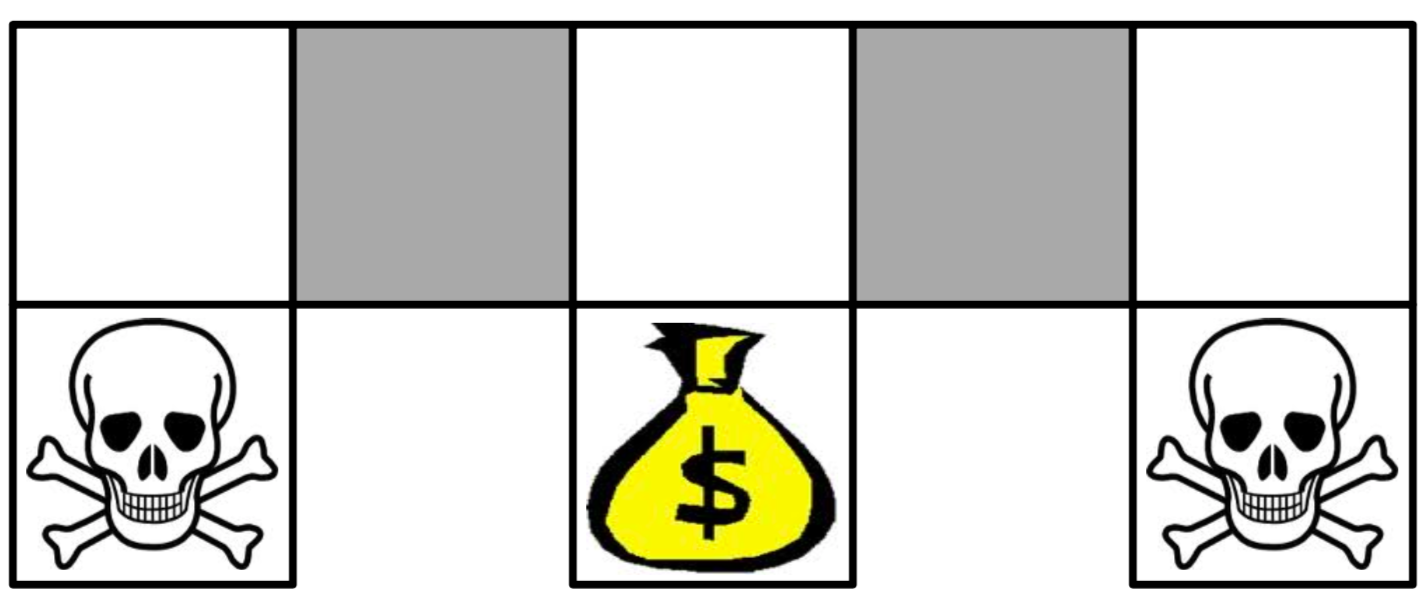
\includegraphics[width=.6\textwidth]{alias}\end{center}
    \begin{itemize}
        \item Main problem: deterministic policy
        \item No good for partially observable environment
        \item The agent cannot differentiate the grey states
        \item An optimal deterministic will either go left or right
    \end{itemize}
\end{frame}

\begin{frame}{Policy Gradient: problem formulation}
    \begin{itemize}
        \item Policy is a function of observation: $\pi_{\theta}(\cdot)$\\\vspace{0.2cm}
        \item Trajectory $\tau$: $\{s_0,a_0,r_0,s_1,a_1,r_1,...\}$ is treated as random variable\\\vspace{0.2cm}
        \item Distribution of $\tau$ is determined by policy $\pi_{\theta}$\\\vspace{0.2cm}
        \item For each trajectory, total reward is defined as $R(\tau)$\\\vspace{0.2cm}
        \item Ultimate goal: optimize expectation $E_{\pi_{\theta}}[R(\tau)]$ w.r.t $\theta$\\\vspace{0.2cm}
    \end{itemize}
\end{frame}

\begin{frame}{Policy Gradient: approximate the gradient}
    \begin{itemize}
        \item What does the gradient look like?
        \begin{equation}
            \label{PG1}
            \begin{split}
            \nabla_\theta E_{\pi_{\theta}}[R(\tau)] &= \nabla_\theta \sum\limits_{\tau} P_\theta(\tau)R(\tau)\\ 
                                                &= \sum\limits_{\tau} \nabla_\theta P_\theta(\tau)R(\tau)\\
                                                &= \sum\limits_{\tau} P_\theta(\tau) \frac{\nabla_\theta P_\theta(\tau)}{P_\theta(\tau)} R(\tau) = E_{\pi_{\theta}}[\nabla_\theta\ln P_\theta(\tau)R(\tau)]\\
            \end{split}
        \end{equation}
        \item Equation \ref{PG1} tell us: gradient can be represented as an expectation\\\vspace{0.2cm}
        \item Why it is important: expectation can be approximated by sampling\\\vspace{0.2cm}
    \end{itemize}
\end{frame}

\begin{frame}{Policy Gradient: approximate the gradient}
    \begin{itemize}
        \item Why the gradient even exists?
            \begin{equation}
                \label{PG2}
                \begin{split}
                    P(\tau) = P(s_0) \prod\limits_{i=0}^\infty \pi_\theta(a_i,s_i) P(s_{i+1} | s_i,a_i)
                \end{split}
            \end{equation}
        \item Assumption: there is an underlying MDP specifying $P(s_{i+1} | s_i,a_i)$ and $P(s_0)$
            \begin{equation}
                \label{PG3}
                \begin{split}
                    \nabla_{\theta}\ln P(\tau) &= \nabla_{\theta}\ln [P(s_0) \prod\limits_{i=0}^\infty \pi_\theta(a_i,s_i) P(s_{i+1} | s_i,a_i)]\\
                                               &= \nabla_{\theta}\ln P(s_0) + \nabla_{\theta}\sum\limits_{i=0}^\infty [\ln \pi_\theta(a_i,s_i)+\ln P(s_{i+1} | s_i,a_i)]\\
                                               &= \nabla_{\theta}\sum\limits_{i=0}^\infty \ln \pi_\theta(a_i,s_i)
                \end{split}
            \end{equation}
    \end{itemize}
\end{frame}


\begin{frame}{Policy Gradient: understanding the formula}
    Combine all equation in previous slides, one important formula:
        \begin{equation}
            \label{PG4}
            \begin{split}
                \nabla_\theta E_{\pi_{\theta}}[R(\tau)] = E_{\pi_{\theta}}[R(\tau)\nabla_\theta\sum\limits_{s_i,a_i \in \tau}\ln\pi_\theta(a_i,s_i)]
            \end{split}
        \end{equation}
    Intuition from equation \ref{PG4}, adjustment magnitude of policy on $\pi_{\theta}(a,s)$:\vspace{0.2cm}
    \begin{itemize}
        \item In proportion to the total reward gained from trajectories containing $(a,s)$\vspace{0.2cm}
        \begin{itemize}
            \item Rationale: good actions lead to good trajectories, while bad actions lead to bad ones\vspace{0.2cm}
            \item What about good actions in trajectories with bad overall performance? work on it later\vspace{0.2cm}
        \end{itemize}\vspace{0.2cm}
        \item In inverse proportion to the probability of performing action $a$ on state $s$\vspace{0.2cm}
        \begin{itemize}
            \item consider actions sampled frequently but with small positive effect\vspace{0.2cm}
            \item mitigate case where 'not-so-good' actions are rewarded frequently\vspace{0.2cm}
        \end{itemize}
    \end{itemize}
\end{frame}


\begin{frame}{Vanilla Policy Gradient: \textbf{REINFORCE}}
    So far, we obtain the first policy gradient algotithm called \href{http://www-anw.cs.umass.edu/~barto/courses/cs687/williams92simple.pdf}{\textbf{REINFORCE}} \textcolor{CUHKgreen}{\footnotesize[Williams, R. J.]}
    \begin{center}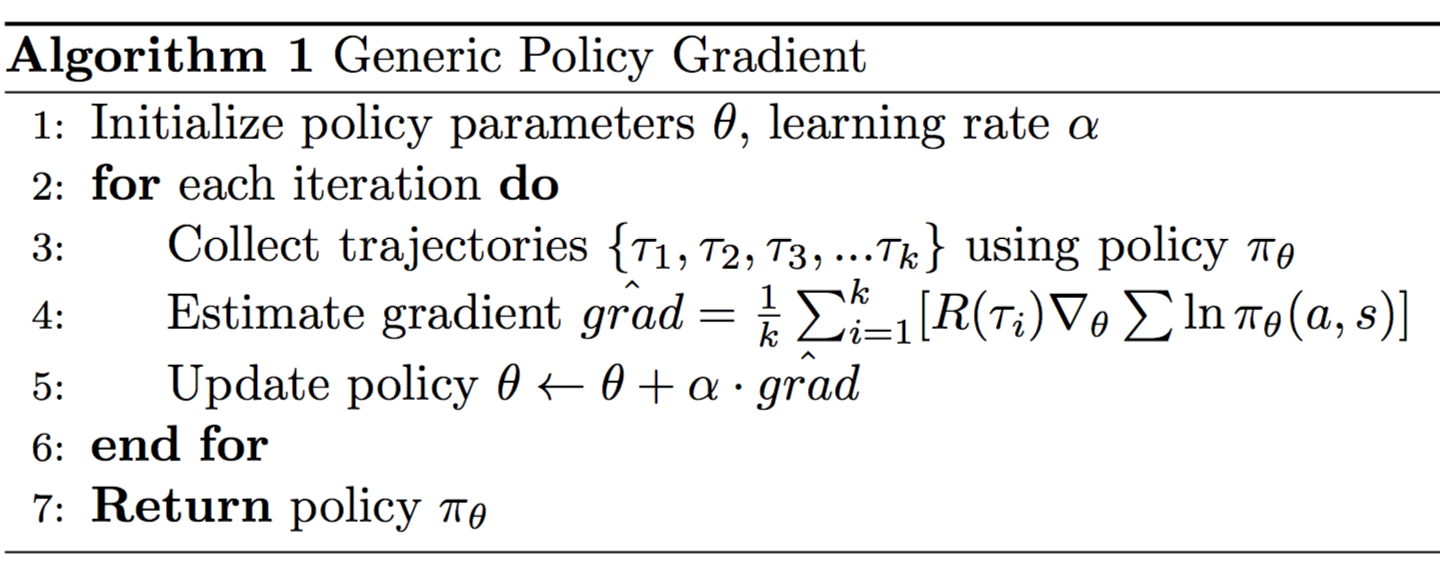
\includegraphics[width=.9\textwidth]{REINFORCE}\end{center}
\end{frame}

\begin{frame}{Vanilla Policy Gradient: \textbf{REINFORCE}}
    \vspace{0.2cm}
    \begin{center}Experiment on CartPole game:\\Bad performance, worse than random play after 1000 episodes of training\\\href{https://www.youtube.com/watch?v=1bvTOM7Az3s}{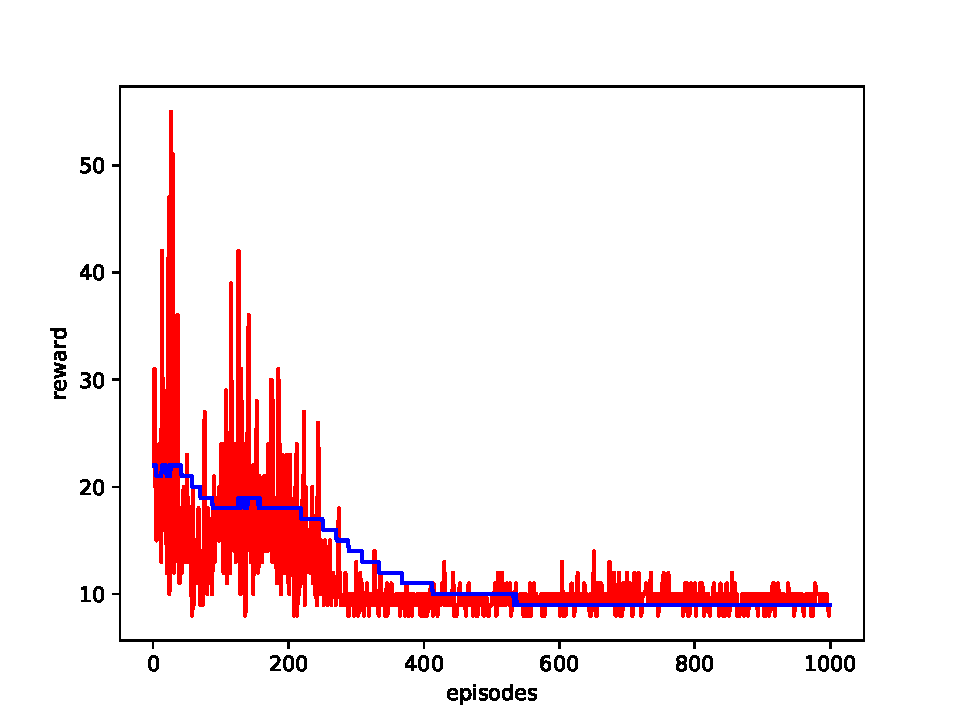
\includegraphics[width=.7\textwidth]{REINFORCE1}}\end{center}
\end{frame}

\begin{frame}{Improvement for \textbf{REINFORCE}: baseline}
    \begin{itemize}
        \item One natural quetion: what if reward is always positive? \\
        \item Do we have to always increase $\pi_{\theta}(a,s)$ because $R(\tau)$ is positive (as in formula \ref{PG4})?\\
        \item Actually, we only cares about the relative performance of trajectories\\
        \item Observation from formula \ref{baseline}: we can remove any constant term $A$ from the expectation with out introducing bias.
        \item $A$ can be the average performance for all trajectories, it is referenced as a baseline
    \end{itemize}
    \begin{equation}
        \label{baseline}
        \begin{split}
            E_{\pi_\theta}[\sum\limits_{a}A\cdot\nabla\ln\pi(a,S)] &= \sum\limits_{a}\pi_\theta(a,S)A\frac{\nabla_\theta\pi_\theta(a,S)}{\pi_\theta(a,S)}\\
                                                                   &= A \sum\limits_{a}\nabla_\theta\pi(a,S)\\
                                                                   &= A\cdot\nabla_\theta\sum\limits_{a}\pi_\theta(a,S)= A \nabla_\theta(1)= 0
        \end{split}
    \end{equation}
    
\end{frame}

\begin{frame}{Improvement for \textbf{REINFORCE}: baseline}
    \vspace{0.2cm}
    \begin{center}Experiment on CartPole game:\\Better than before: an upgoing trend of rewards\\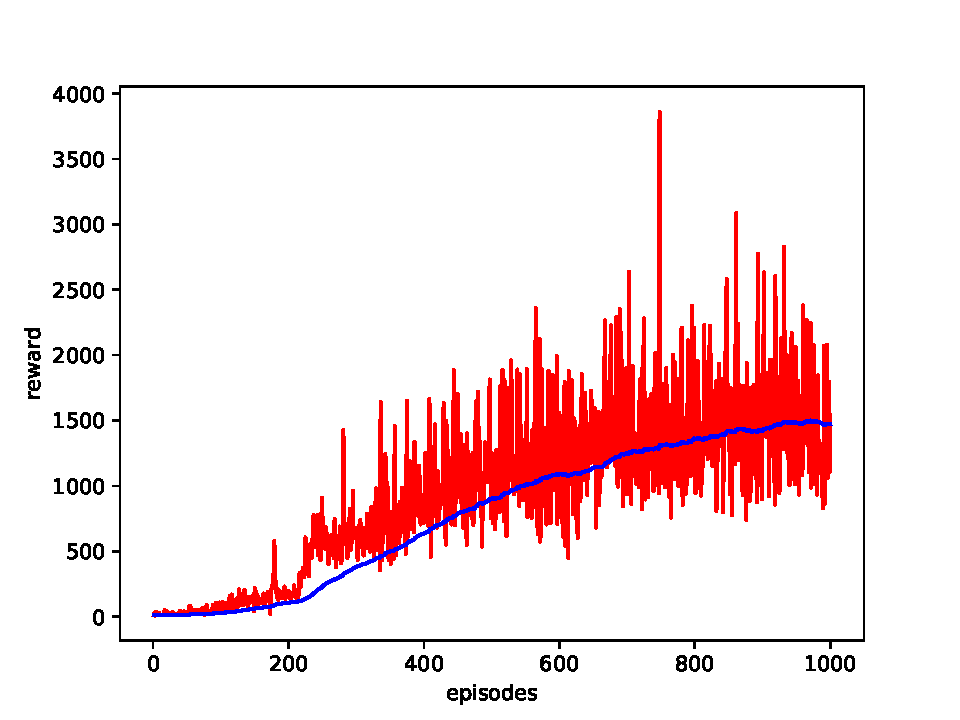
\includegraphics[width=.7\textwidth]{baseline_REINFORCE}\end{center}
\end{frame}

\begin{frame}{Improvement for \textbf{REINFORCE}: advantage function}
    \begin{itemize}
        \item Why we award/punish an action (s,a) based on the entire trajectory reward?\\
        \item Markov property: the action $a_t$ only affects rewards after time $t$.
        \begin{equation}
            \label{indp}
            \begin{split}
                E_{\pi_\theta}[R_{0:i-1}(\tau)\nabla_\theta\ln\pi_\theta(a_i,s_i)] = 0
            \end{split}
        \end{equation}  
        \item Actually, we can exploit the markov property to refine formula \ref{PG4}
            \begin{equation}
                    \label{refinePG1}
                    \begin{split}
                        \nabla_\theta E_{\pi_{\theta}}[R(\tau)] &=E_{\pi_{\theta}}[\sum(\nabla_\theta\ln\pi_\theta(a_i,s_i)(R_{0:i-1}(\tau)+R_{i:\infty}(\tau)))]\\
                        &=E_{\pi_{\theta}}[\sum(\nabla_\theta\ln\pi_\theta(a_i,s_i)R_{i:\infty}(\tau))]\\
                    \end{split}
            \end{equation}
        \item Recall that subtraction of baseline doesn't change the expectation
        \begin{equation}
                    \label{refinePG2}
                        \nabla_\theta E_{\pi_{\theta}}[R(\tau)] = E_{\pi_{\theta}}[\sum\nabla_\theta\ln\pi_\theta(a_i,s_i)(R_{i:\infty}(\tau)-V_{\pi_\theta}(s_i))]
        \end{equation}

    \end{itemize}  
\end{frame}

\begin{frame}{Improvement for \textbf{REINFORCE}: advantage function}
    \begin{itemize}
    \item As shown in equation \ref{refinePG2}, $R_{i:\infty}(\tau)-V_{\pi_\theta}(s_i)$ is the actual term that determines the magnitude we adjust probability $\pi_{\theta}(a_i,s_i)$\vspace{0.3cm}
    \item $R_{i:\infty}(\tau)-V_{\pi_\theta}(s_i)$ is also known as the advantage function \vspace{0.3cm}
    \item Rationale: extra reward gained when performing certain action $a_i$ on state $s_i$ compared to average reward from that state under policy $\pi_{\theta}$\vspace{0.3cm}
    \end{itemize}
\end{frame}

\begin{frame}{Improvement for \textbf{REINFORCE}: advantage function}
    \vspace{0.2cm}
    \begin{center}Experiment on CartPole game:\\Only after 141 episodes of training, surviving time boosted to 20k! \\\href{https://youtu.be/6EdXsW5A1iU}{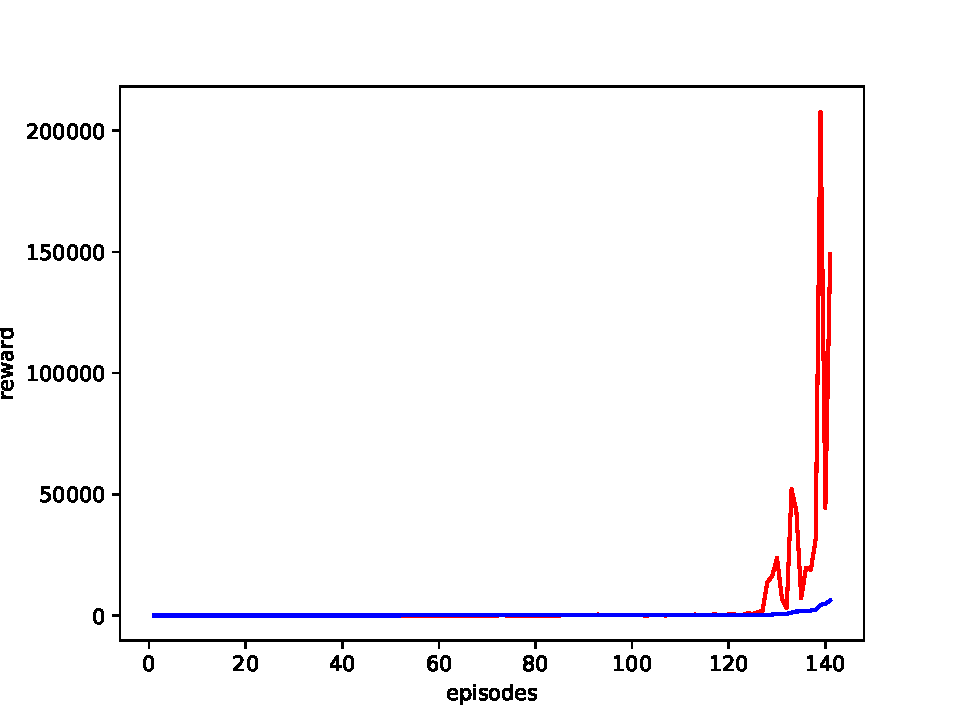
\includegraphics[width=.7\textwidth]{adv_REINFORCE}}\end{center}
\end{frame}

\begin{frame}{Actor-Critic: a combination}
    So far, we mainly focused on pure value-based and pure policy-based methods ... \vspace{0.3cm}
    \begin{itemize}
        \item Value-based: problem of deterministic policy in partially observed environments\vspace{0.3cm}
        \item Policy-based: credit assignment problem (delay between action and reward)\vspace{0.3cm}
        \item Why not combine them?\vspace{0.3cm}
        \item Still use policy function\vspace{0.3cm}
        \item Also adopt an estimator for state values to approximate advantage function\vspace{0.3cm}
        \item Policy updates without delay!
    \end{itemize}
\end{frame}

\begin{frame}{Actor-Critic: algorithm}
    \vspace{0.2cm}
    Now there are two function to learn: policy function $\pi_{\theta}$ is known as actor and value estimator $\hat{V_{\varphi}}$ is known as critic, hence the model named \textbf{Actor-Critic}.
    \begin{center}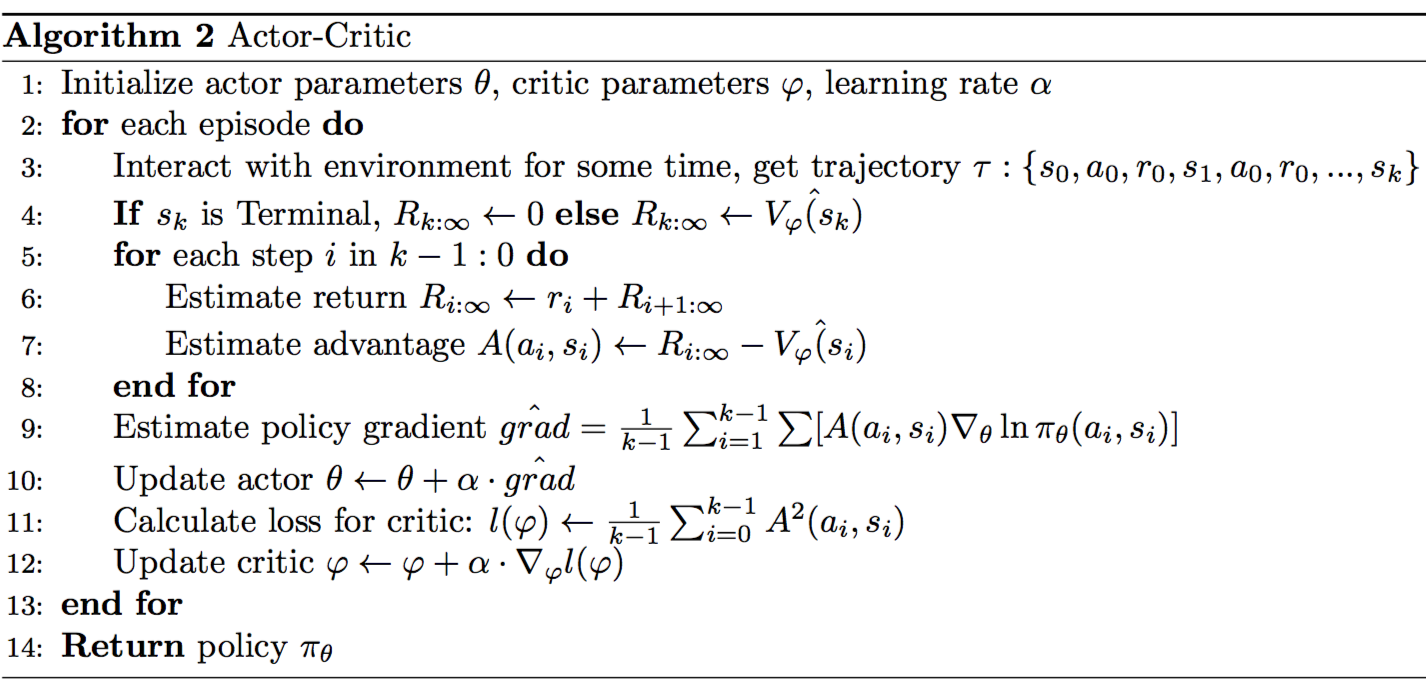
\includegraphics[width=.8\textwidth]{AC1}\end{center}
\end{frame}

\begin{frame}{Further improvement: clipped objective function}
    \begin{itemize}
        \item In previous section, policy gradient method works by computing gradient estimator in form
            \begin{equation}
                \label{commonPG}
                \hat{g} = \hat{E_t}[\nabla_{\theta}\ln\pi_\theta(a_t,s_t)\hat{A}_{t}]
            \end{equation}
        \item The estimator $\hat{g}$ can be obtained by differentiating the objective
            \begin{equation}
                \label{objPG}
                L^{PG}(\theta) = \hat{E_t}[\ln\pi_\theta(a_t,s_t)\hat{A}_{t}]
            \end{equation}
        \item Multiple steps to optimize $L^{PG}$ on same trajectory: destructively large policy updates \textcolor{CUHKgreen}{\footnotesize[Schulman, John et al.]}. 
        \item To improve sample efficiency, they adopt strategy of clipping the surrogate objective function in form $L^{CPI}(\theta)$:

    \end{itemize} 
\end{frame}

\begin{frame}{Further improvement: clipped objective function}
\begin{equation}
                \label{objPPO}
                L^{CPI}(\theta) = \hat{E_t}[\frac{\pi_\theta(a_t,s_t)}{\pi_{\theta_{old}}(a_t,s_t)}\hat{A}_{t}]
            \end{equation}
\begin{itemize}
    \item $\pi_{\theta_{old}}$: fixed term generated by old policy\vspace{0.2cm}
    \item $\pi_{\theta}$: current policy being optimized. \vspace{0.2cm}
    \item The ratio $\frac{\pi_\theta(a_t,s_t)}{\pi_{\theta_{old}}(a_t,s_t)}$ is denoted as $r_t(\theta)$\vspace{0.2cm}
    \item $r_t(\theta)$ measures the difference between current policy and old policy\vspace{0.2cm}
    \item we don't want too big a update step, hence some constraint based on $r_t(\theta)$\vspace{0.2cm}
    \item In practise we use the gradient of following objective function\vspace{0.2cm}
\end{itemize}
\begin{equation}
    \label{clipPPO}
    L^{CLIP}(\theta) = \hat{E_t}[\min(r_t(\theta)\hat{A_t},\mathrm{clip}(r_t(\theta),1-\epsilon,1+\epsilon)\hat{A_t}]
\end{equation}
\end{frame}

\begin{frame}{Proximal Policy Optimization(PPO)}
    \vspace{0.15cm}
    The algorithm is known as \href{https://arxiv.org/pdf/1707.06347.pdf}{Proximal Policy Optimization} \textcolor{CUHKgreen}{\footnotesize[Schulman, John et al.]}\\\vspace{0.15cm}
    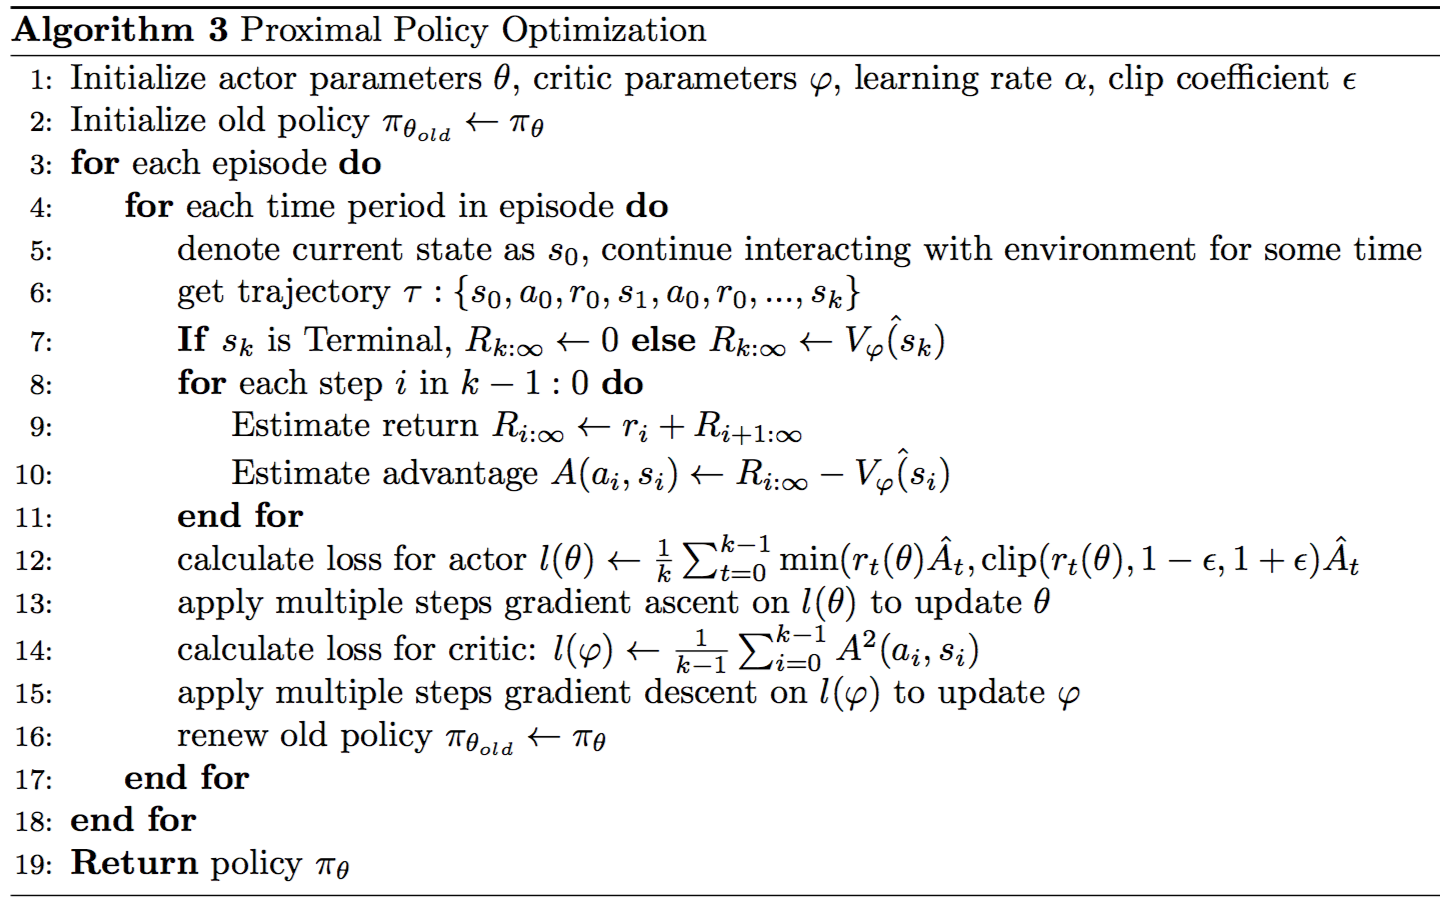
\includegraphics[width=.8\textwidth]{PPO1}
\end{frame}

\begin{frame}{Proximal Policy Optimization(PPO): some demo}
    \vspace{0.15cm}
    Test on \href{https://gym.openai.com/}{OpenAI gym} Agents implemented and trained using \href{https://en.wikipedia.org/wiki/PyTorch}{Pytorch}\\\vspace{0.15cm}
    For detailed information about task environment, check \href{https://github.com/openai/gym/wiki/Table-of-environments}{this list}\\\vspace{0.15cm}
    \begin{itemize}
        \item CartPole-v0: \href{https://www.youtube.com/watch?v=1bvTOM7Az3s}{no training} and \href{https://www.youtube.com/watch?v=l1gOoNFSq8E}{trained}
        \item MountainCar-v0: \href{https://www.youtube.com/watch?v=SAGHdqGvbzA}{no training} and \href{https://www.youtube.com/watch?v=6wYzj74x_l4}{trained}
        \item LunarLander-v2: \href{https://www.youtube.com/watch?v=ZFmx0l6Pe60}{no training} and \href{https://www.youtube.com/watch?v=BysTYEG4fDE}{trained}
        \item Pendulum-v0: \href{https://www.youtube.com/watch?v=bxojAfY5PPw&t=5s}{no training} and \href{https://www.youtube.com/watch?v=yasKyY3hE88}{trained}
    \end{itemize}
    Some strategyies in our training:\\\vspace{0.15cm}
     \begin{itemize}
        \item For continous action space (like Pendulum-v0): discretize it
        \item Set a maximum number (5000) of steps for each episode during training
        \item Use a large batch size (512) to perform gradient descent
        \item Adopt different step size for Actor and Critic updates
        \item Have a look at \href{https://github.com/JamesTuna/RL_collects/blob/master/PPO/PPO.py}{our code} on github
    \end{itemize}
\end{frame}



\begin{frame}{Further improvement: high score buffer replay}
    \begin{itemize}
        \item The learning curve is like:\\\vspace{0.2cm}
        \begin{center}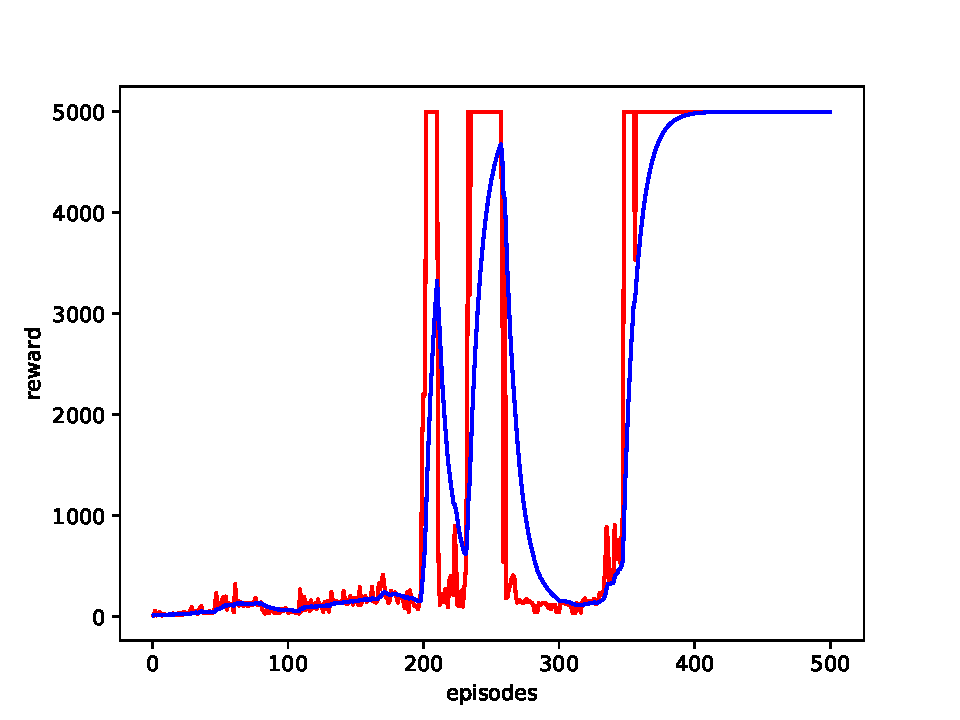
\includegraphics[width=.7\textwidth]{no_buffer}\end{center}
    \end{itemize}  
\end{frame}



\begin{frame}{Further improvement: high score buffer replay}
    \begin{itemize}
        \item A Typical training curve in Reinforcement Learning\\\vspace{0.2cm}
        \item Not stable: immature policy, more frequent explorational moves\\\vspace{0.2cm}
        \item Another problem: cases where positive signals are extremely rare\\\vspace{0.2cm}
        \item Idea comes naturally: store those trajectories with high score in a buffer\\\vspace{0.2cm}
        \item Use importance sampling to learn from high score buffer from time to time\\\vspace{0.2cm}
    \end{itemize}  
\end{frame}

